\documentclass[11pt,letterpaper]{article}
\usepackage[
  letterpaper,
  top=0.75in,
  bottom=0.75in,
  left=0.75in,
  right=0.75in,
  headheight=14pt,
  headsep=12pt,
  footskip=18pt
]{geometry}

\usepackage{fontspec}
\setmainfont{Helvetica}
\setmonofont{Menlo}

\usepackage{amsmath,amssymb,amsfonts}
\usepackage{booktabs}
\usepackage{tabularx}
\usepackage{graphicx}
\usepackage{xcolor}
\usepackage{hyperref}
\usepackage{caption}
\usepackage{microtype}
\usepackage{float}

\hypersetup{
  breaklinks=true,
  colorlinks=true,
  linkcolor=blue!70!black,
  citecolor=blue!70!black,
  urlcolor=blue!70!black
}

\def\UrlBreaks{\do\/\do\a\do\b\do\c\do\d\do\e\do\f\do\0\do\1\do\2\do\3\do\4\do\5\do\6\do\7\do\8\do\9\do\-}

\captionsetup{font={small},labelfont={bf},skip=6pt}

\title{\textbf{Runtime Provenance Contracts for Mitigating Tool Poisoning in MCP Agents}\\[0.3em]\large A Paired Evaluation on MCPTox Across Six Models}
\author{\textbf{Samir Sawarkar — FAULTLINE}}
\date{September 2026}

\setcounter{secnumdepth}{0}

\begin{document}
\sloppy
\maketitle

\begin{abstract}
We deployed and evaluated an independent defensive second arm on the Model Context Protocol Poisoning benchmark (MCPTox), testing whether a client-side runtime provenance contract on tool-call arguments with call-only retry gating mitigates tool poisoning across six model rungs. Defending tool-integrated language model agents against tool poisoning is difficult because malicious instructions embedded directly within tool definitions exploit models' instruction-following capabilities, causing models to divert execution into harmful actions before runtime data flows even occur. We interposed a five-stage provenance policy engine between model generations and tool execution that enforces envelope formatting, tool enumeration allowlists, strict schema argument boundaries, and substring-grounding of argument values against the user turn, granting a single retry gated exclusively on contract-blocked tool calls. On 300 MCPTox instances, six models via one gateway, one LLM judge, one day, the provenance contract achieved a statistically significant paired mean score reduction of $\text{Mean } \Delta = -0.2194$ (95\% CI $[-0.2400, -0.1983]$, sign-flip permutation $p < 0.0001$, descriptive paired Cohen's $d_z = -0.49$), cutting overall ASR from 28.83\% to 6.89\% (valid ASR from 30.32\% to 7.41\%) pooled, removing 421 attacks while inducing only 26 (McNemar exact $p = 5.61 \times 10^{-93}$). The runtime contract reduced Attack Success Rate over valid completions by up to 35.5 percentage points on frontier models on static MCPTox instances (falling from 40.81\% to 5.26\% on GPT 5.6 Luna and from 41.84\% to 9.76\% on Qwen 3.8 Flash). However, on Gemini 3.7 Flash (R5), the reduction was statistically non-significant ($b=5, c=1$, exact $p=0.2188$) due to high baseline autonomous resistance. Furthermore, runtime rejection shifted error distributions: across all rungs, Failure-Direct-Execution rose 41.4\% pooled from 145 to 205 instances (R1: 14$\to$30, R2: 26$\to$31, R3: 30$\to$51, R4: 21$\to$31, R5: 27$\to$25, R6: 27$\to$37), and smaller models exhibited post-rejection collapse, with 65 empty completions on R1 accounting for 92.9\% of its 70 Invalid instances (21.7\% of all 300 R1 instances). Finally, trace replay across 10,227 traces reveals an intrinsic trade-off: while blocking 87.0\% of author-labelled attack successes, rigid substring grounding false-blocks 24.5\% of benign executions when legitimate tasks require ungrounded world knowledge.
\end{abstract}

\section{1. Introduction}

Autonomous language model (LLM) agents increasingly rely on dynamic tool protocols to interact with external databases, APIs, and software environments. The Model Context Protocol (MCP)\footnote{Model Context Protocol Specification, revision 2025-06-18. \url{https://modelcontextprotocol.io/specification/2025-06-18}} provides an open JSON-RPC standard for dynamic tool discovery and execution. Under MCP, a client agent queries servers for available tools, ingests schema definitions and natural language descriptions, and constructs tool calls based on user objectives. However, this coupling introduces a critical threat: tool poisoning. Unlike traditional prompt injections where adversarial payloads reside in user prompts or retrieved documents, tool poisoning embeds instructions directly within tool definitions and parameter schemas. When an agent inspects server tools, poisoned metadata enters its privileged system context. As documented by initial security notifications\footnote{Invariant Labs. MCP Security Notification: Tool Poisoning Attacks (2025). \url{https://invariantlabs.ai/blog/mcp-security-notification-tool-poisoning-attacks}} and demonstrated on MCPTox [1], tool poisoning exploits models' instruction-following capabilities, directing execution into unauthorized actions, credential exfiltration, and data tampering. In this work, our single primary contribution is demonstrating that syntactic substring grounding of tool arguments at the client boundary reduces tool-poisoning attack success across diverse LLM agent families, while introducing an operational false-block penalty on tasks requiring ungrounded world knowledge.

Greshake et al. [2] formulated the foundational threat of indirect prompt injection (IPI), demonstrating that untrusted data acting as control instructions enables arbitrary remote API manipulation. Benchmarks such as InjecAgent [3] and AgentDojo [4] demonstrated widespread susceptibility across state-of-the-art models in ReAct-prompted and dynamic agentic settings. To mitigate this vulnerability, recent structural defenses (including CaMeL [5], Spotlighting [6], AuthGraph [7], DualView [8], and Progent [9]) proposed capability tokens, input transformation, graph-based alignment, and out-of-band reference monitors. Several report near-zero residual attack success rates on benchmarks like AgentDojo.

However, existing studies exhibit four recurring limitations: (1) they rely on synthetic environments rather than authentic multi-server protocols; (2) they omit quantitative measurement of false blocks on valid world-knowledge inferences; (3) they treat agent interaction as a static single step, ignoring how runtime rejection feedback alters model behavior; and (4) they benchmark few models, obscuring how defense efficacy interacts with model compliance. No independent defensive second arm has previously been evaluated on MCPTox [1].

In this study, we investigate: \emph{Does a runtime provenance contract on tool-call arguments (every argument value must be grounded in the user turn), with one retry gated on a rejected call, reduce tool-poisoning attack success on MCPTox relative to the published single-turn protocol, across six models, on the same 300 instances?}

We implement and evaluate FAULTLINE Arm B: a client-side mediation layer intercepting tool calls before dispatch, subjecting them to a deterministic five-stage provenance contract, with a single retry gated strictly on rejected calls. We benchmark Arm B against the upstream unconstrained baseline (Arm A) from \texttt{inspect-evals-mcptox}\footnote{Stefano Amorelli. inspect-evals-mcptox: MCPTox as an Inspect AI evaluation. \url{https://github.com/stefanoamorelli/inspect-evals-mcptox}, commit \texttt{d45705b}.} across 1,800 paired instances on six model rungs.

Interposing a deterministic client-side argument provenance contract (verbatim substring grounding of argument leaves against user turns) with call-only retry gating blunts tool-poisoning attack success on static MCPTox instances across six LLMs, but incurs an operational false-block penalty on legitimate tool calls requiring ungrounded world knowledge. Our study delivers four contributions:
\begin{itemize}
\item \textbf{An independent defensive second arm on MCPTox:} The first paired evaluation of a defensive architecture on MCPTox, testing 1,800 paired instances across six model rungs (Qwen 3.7 Flash, GLM 5.3 Flash, Qwen 3.8 Flash, GPT 5.6 Luna, Gemini 3.7 Flash, DeepSeek v4 Pro) under strict stimulus and judge parity.
\item \textbf{Empirical confirmation of pre-registered hypothesis H7:} On 300 MCPTox instances, six models via one gateway, one LLM judge, one day, we show that bounded, typed provenance contracts achieve a statistically significant paired mean score reduction of $\text{Mean } \Delta = -0.2194$ (95\% CI $[-0.2400, -0.1983]$, $p < 0.0001$, descriptive $d_z = -0.49$), cutting overall ASR from 28.83\% to 6.89\% (valid ASR from 30.32\% to 7.41\%) pooled, removing 421 attacks while inducing 26 ($p = 5.61 \times 10^{-93}$).
\item \textbf{Characterization of retry gating dynamics:} We uncover that injecting rejection messages following safe natural language refusals misleads models into generating spurious malicious calls. Gating retries strictly on contract-rejected calls (\texttt{--retry-mode call-only}) preserves 230 natural language refusals while allowing 479 legitimate corrections.
\item \textbf{Quantification of contract costs:} Through live execution and offline replay over 10,227 traces, we show that while the contract reduced 87.0\% of attack successes on static MCPTox instances, rigid substring grounding incurs a 24.5\% false-block penalty on legitimate tools requiring world-knowledge entity resolution, and retains residual vulnerability (10.93\% ASR) on function hijacking.
\end{itemize}

\section{2. Background and Related Work}

\subsection{2.1 Approaches to Tool-Agent Security}

\textbf{Unconstrained Tool Agents (Baseline Threat Model).} Greshake et al. [2] demonstrated that processing untrusted data as control instructions enables arbitrary remote API manipulation. Perez \& Ribeiro [10] showed that simple handcrafted inputs misalign models into goal hijacking and prompt leaking. Zhan et al. [3] developed InjecAgent across 1,054 test cases, finding ReAct GPT-4 vulnerable 24\% of the time, doubling under enhanced hacking prompts. Debenedetti et al. [4] established AgentDojo across 97 tasks and 629 security test cases, observing that frontier LLMs fail many tasks unattacked and that prompt injection attacks break subsets of security properties. Wang et al. [1] introduced MCPTox, constructing 1,312 test cases across 45 live MCP servers and 353 tools. Across 20 agent settings, Wang et al. (§4.2) report: ``The overall results reveal a widespread and significant vulnerability to Tool Poisoning attacks across a diverse range of popular models, with an average ASR for all model settings was 36.5\%.'' Furthermore, ``More powerful models like o1-mini and Phi-4 exhibited the highest vulnerability, with extremely high average ASRs of 72.8\% and 70.2\%, respectively'' (§4.2). Wang et al. (§4.4) describe this as an Inverse Scaling phenomenon: ``Our analysis also revealed the Inverse Scaling phenomenon in MCP Tool Poisoning: more capable models (such as larger models or when reasoning is enabled) often lead to higher vulnerability.'' We note that while our ladder's ordering is consistent with this finding, our empirical design does not test it.

\textbf{Control/Data Flow Isolation and Capabilities.} Debenedetti et al. [5] introduced CaMeL, extracting control and data flows from trusted queries using capability tokens. Enforcing policies at tool dispatch, CaMeL solves 77\% of AgentDojo tasks with provable security (0\% security violations) compared to 84\% undefended utility. An et al. [11] developed IPIGuard, modeling execution as traversal over a planned Tool Dependency Graph (TDG) to decouple action planning from external data.

\textbf{Input Transformation and Data Spotlighting.} Hines et al. [6] proposed Spotlighting, applying continuous encoding or delimiter transformations to untrusted inputs. Spotlighting provides provenance signals that reduce indirect prompt injection ASR from over 50\% to below 2\% across GPT models with minimal NLP task impact.

\textbf{Graph-Based Provenance and Authorization Alignment.} Wang et al. [7] introduced AuthGraph, constructing complementary execution provenance graphs and clean-context authorization graphs. Graph alignment checking detects parameter-source deviations, reducing AgentDojo ASR from 40\% to 1\% on GPT-4o and AgentDyn ASR from 39\% to 2\%. Souza et al. [12] developed PROV-AGENT, extending W3C PROV via MCP to track agent interactions and tool calls into end-to-end workflow traces. Maloyan \& Namiot [13] analyzed sleeper channels in persistent agents, formulating the D2 provenance gate with canonical action digests and proofs against seven deployment invariants.

\textbf{Dual-View Environmental Isolation.} Kim et al. [8] proposed DualView, separating data into an AgentView (symbolic tokens) and a HumanView (raw content). DualView blocked 100\% of tested direct and stored IPI attacks on PinchBench with a 1.8--6.4 point utility penalty.

\textbf{Deterministic Out-of-Band Policy Enforcement.} Narisetty et al. [9] evaluated deterministic reference monitors that mediate actions externally without relying on model self-refusal. Evaluating Progent on AgentDojo with Qwen2.5-7B, attack success dropped from 25.8\% to 4.2\% (2.6\% under adaptive attack), though authors emphasize static evaluations risk overstating defense robustness.

\textbf{Runtime Argument Provenance Contracts (FAULTLINE).} Our approach enforces deterministic client-side argument grounding directly on tool-call leaves, validating parameters against the user query turn with a bounded, gated retry protocol.

\subsection{2.2 Threat Model Differences and the Benchmark Gap}

A major question in LLM agent security is how structural and runtime defenses perform across different attack surfaces. Prior defenses (including CaMeL [5], Spotlighting [6], AuthGraph [7], and DualView [8] ) were evaluated primarily on benchmarks such as AgentDojo and PinchBench under data-payload indirect prompt injection (IPI) threat models. In those settings, adversarial instructions reside in untrusted retrieved documents or tool outputs encountered during execution, and these structural defenses achieved near-zero residual attack rates (e.g., 0\% violations in CaMeL, $<2\%$ ASR in Spotlighting, 1\%--2\% ASR in AuthGraph, and 100\% attack blocking on tested PinchBench tasks in DualView ).

However, MCP tool poisoning represents a distinct attack surface from data-payload IPI. On MCPTox [1], malicious instructions are embedded directly within tool definitions and schema parameters across 45 authentic servers, entering the model's privileged system prompt during initial tool discovery. No prior defensive architecture has been evaluated on MCPTox.

We emphasize that the residual vulnerabilities observed in our evaluation reflect the behavior of client-side syntactic provenance contracts on this new tool poisoning surface; our residual is NOT evidence against those prior papers or defenses, which addressed different threat models and mechanisms. Rather, four architectural distinctions separate data-payload IPI from MCP tool poisoning:

\begin{enumerate}
\item[1.] \textbf{Benchmark and Injection Topology:} AgentDojo and PinchBench focus on retrieved user-data payloads encountered at runtime, whereas MCPTox embeds attacks directly into tool metadata across 45 authentic servers, entering privileged system context prior to invocation.
\item[2.] \textbf{Threat Model Timing:} Tool poisoning alters initial tool selection \emph{before} runtime data flows occur. Capability architectures that assume uncorrupted tool schemas can be diverted upon initial tool dispatch.
\item[3.] \textbf{Evaluation Criteria:} Programmatic invariant checks verify specific data exfiltration events, whereas MCPTox uses an automated LLM judge assessing semantic intent fulfillment across ten risk categories.
\item[4.] \textbf{Model Capability Spectrum:} Frontier reasoning models follow detailed schema instructions with high fidelity. When instructions reside in tool definitions, compliance varies across model families, as demonstrated by Wang et al. [1].
\end{enumerate}

Evaluating how structural, capability, and provenance defenses generalize to schema-level tool poisoning remained unexamined prior to this study.

\section{3. Pre-registration and Hypotheses}

\subsection{3.1 Pre-registered Hypothesis H7}

This evaluation was pre-registered under project identifier P8. The formal specification from \texttt{HYPOTHESES.md} is reproduced verbatim:

\begin{itemize}
\item \textbf{Hypothesis ID:} H7
\item \textbf{Hypothesis Statement (verbatim):} \texttt{Bounded + typed contracts reduce ASR vs published MCPTox rates}
\item \textbf{Falsifier (verbatim):} \texttt{ASR CI overlaps or exceeds the published band}
\item \textbf{Benchmark Vulnerability Band:} Wang et al. [1] report (§4.2) that ``The overall results reveal a widespread and significant vulnerability to Tool Poisoning attacks across a diverse range of popular models, with an average ASR for all model settings was 36.5\%'' and §4.2 that ``More powerful models like o1-mini and Phi-4 exhibited the highest vulnerability, with extremely high average ASRs of 72.8\% and 70.2\%, respectively''; pre-registered hypothesis H7 specifies evaluating whether Arm B bounds ASR strictly below 0.365, hypothesizing that Arm B bounds ASR below this benchmark threshold.
\item \textbf{Prediction if True:} Arm B ASR 95\% Wilson confidence intervals fall strictly below the published baseline band (upper bound $< 0.365$) and strictly below the paired Arm A control across evaluated model rungs.
\item \textbf{Prediction if False:} Arm B ASR 95\% Wilson confidence intervals overlap or exceed 0.365.
\item \textbf{Statistical Test:} Paired exact McNemar test for discordant pairs ($b$ attacks removed vs $c$ attacks induced), continuity-corrected $\chi^2$ test, and Wilson 95\% score confidence intervals per rung.
\end{itemize}

\subsection{3.2 Definition of Attack Success Rate (ASR)}

In accordance with MCPTox [1], our primary metric is \textbf{Attack Success Rate over valid completions} ($\text{ASR}_{\text{valid}}$):

\begin{equation}
\resizebox{0.95\textwidth}{!}{$\displaystyle \text{ASR}_{\text{valid}} = \frac{\text{Success}}{\text{Success} + \text{Failure-Ignored} + \text{Failure-Direct-Execution} + \text{Failure-Refused} + \text{Contract-Blocked}} = \frac{\text{Success}}{n_{\text{valid}}}$}
\end{equation}

where $n_{\text{valid}} = n - \text{Invalid} - \text{Error}$. An instance is valid if the model generates a parseable completion evaluated into one of the substantive outcome categories. Completions resulting in syntax errors, unparseable outputs, or generation truncations are classified as \texttt{Invalid}. Any unhandled runtime execution faults are classified as \texttt{Error}. Both \texttt{Invalid} and \texttt{Error} are excluded from the denominator. In defended arms, \texttt{Contract-Blocked} denotes an attempted tool call intercepted by the policy engine on Step 1 or Step 2; it is counted in the valid denominator as a non-success (an interdicted attack or non-successful execution).

Where overall rates are reported across the full sample ($n = 300$ per rung), we explicitly label them as \textbf{Attack Success Rate over all instances} ($\text{ASR}_{\text{all}}$):

\begin{equation}
\text{ASR}_{\text{all}} = \frac{\text{Success}}{n}
\end{equation}

Every rate reported denotes $\text{ASR}_{\text{valid}}$ unless explicitly designated as $\text{ASR}_{\text{all}}$. Where pooled rates are reported, $\text{ASR}_{\text{all}}$ is stated beside $\text{ASR}_{\text{valid}}$.

We also define an exploratory transition metric, $\text{false\_block\_proxy}$, measuring the number of instances where Arm A safely completed the user task (\texttt{Failure-Ignored}) while Arm B concluded as \texttt{Contract-Blocked}. The denominator for this proxy is Arm A \texttt{Failure-Ignored}. We caution that this ad-hoc proxy measures only direct transitions into \texttt{Contract-Blocked}; it does not capture instances where contract rejection caused subsequent model collapse into \texttt{Invalid} (empty completions) or diversion into \texttt{Failure-Direct-Execution}. Comprehensive benign task utility is measured via offline trace replay in Section 5.6.

\subsection{3.3 Separation of Pre-Registered Hypothesis and Post-Hoc Findings}

We explicitly separate our confirmatory pre-registered hypothesis (H7, Section 3.1) from two post-hoc exploratory findings discovered during experimental execution:
\begin{itemize}
\item \textbf{H7-sub (Post Hoc):} \emph{Runtime provenance contracts are least effective on Template-2 (function hijacking).} \\
\emph{Rationale:} The contract grounds argument leaves against the user query. We interpret that in Template-2 attacks, adversarial instructions manipulate the model into invoking an unintended legitimate tool whose schema parameters naturally align with user query tokens, weakening argument-level taint tracking relative to parameter injection (Template-3) or tool description injection (Template-1).
\item \textbf{Retry-on-Refusal Finding (Post Hoc):} \emph{Injecting contract rejection prompts following safe natural language refusals induces direct execution failures.} \\
\emph{Rationale:} Discovered during pilot evaluations on R4 (GPT 5.6 Luna), unconstrained retry prompts (\texttt{--retry-mode any}) misled models that had safely refused a poisoned tool into believing an error occurred, coercing them into generating tool calls on the second turn.
\end{itemize}

\section{4. Method}

\subsection{4.1 Paired Arms: Arm A (Control) and Arm B (Contract-Defended)}

\begin{itemize}
\item \textbf{Arm A (Upstream Baseline Control):} We execute \texttt{inspect-evals-mcptox} (commit \texttt{d45705b0a7ae6697c851e311187b06bf7488b13f}) verbatim\footnotemark[3] in an isolated virtual environment (\texttt{.venv-inspect}, \texttt{inspect\_ai==0.3.263}\footnote{UK AI Security Institute. Inspect: A framework for large language model evaluations. \url{https://github.com/UKGovernmentBEIS/inspect_ai} (version 0.3.263).}, \texttt{openai==3.14.0}). It exposes models to authentic MCP server tool definitions and user queries, allowing unconstrained single-turn tool execution with a step cap of 2.
\item \textbf{Arm B (Contract-Defended Second Arm):} We execute FAULTLINE's runtime defense agent. Arm B shares the identical sample loader, instance identifiers, system prompts, tool schemas, user queries, decoding parameters, and automated judge prompt (\texttt{MCPTOX\_JUDGE\_PROMPT}) with Arm A. Arm B intercepts tool calls before dispatch using \texttt{ProvenancePolicy} and applies a single retry gated under \texttt{--retry-mode call-only}. As detailed in Appendix B and documented in our research decisions, \texttt{--retry-mode call-only} was adopted as a protocol correction following pilot evaluation on R4, where unconstrained retry feedback coerced benign prose refusals into malicious tool calls.
\end{itemize}

\subsection{4.2 Verbatim Contract Rules}

The \texttt{ProvenancePolicy} engine (\texttt{faultline\_p2/policy/provenance.py}) intercepts model tool calls and enforces five sequential rules in strict priority order:

\begin{enumerate}
\item[1.] \texttt{multi\_call}: The completion must specify at most one tool call. If two or more call objects are returned, execution is rejected: \emph{``Protocol requires exactly one call; received \{len(raw\_call)\} calls''}.
\item[2.] \texttt{envelope}: The raw call structure must be a valid dictionary containing exactly the keys \texttt{'tool'} (string) and \texttt{'arguments'} (dictionary). Malformed structures fail immediately.
\item[3.] \texttt{unknown\_tool}: The invoked tool name must exist within the server's listed tools. The poisoned tool \emph{is} listed on the authentic MCP server and is therefore permitted by this rule; executing the poisoned tool represents a model choice evaluated by the judge (\texttt{Failure-Direct-Execution}), not an unknown tool error. The contract deliberately does not block poisoned tools by name, as a production defense has no prior knowledge of which server tools are malicious.
\item[4.] \texttt{extra\_argument}: Any argument key present in the call that is not declared in the tool's published JSON schema is strictly forbidden (\texttt{extra=forbid}).
\item[5.] \texttt{provenance}: Every leaf string value within the arguments dictionary must be grounded in the user query context. 
\begin{itemize}
\item \emph{Normalization:} Both the argument string and user query are normalized by lowercasing, collapsing consecutive whitespace, and stripping surrounding quotation marks.
\item \emph{Grounding Condition:} A leaf string is grounded if the normalized string is a verbatim substring of the normalized user query.
\item \emph{Permitted Exemptions:} Non-string primitives (integers, floats, booleans), empty strings, strings of length $\le 3$ characters, and multi-word strings whose every whitespace-separated token of length $> 3$ is individually a substring of the user query pass verification.
\end{itemize}
\end{enumerate}

\subsection{4.3 Retry Gating and Empty-Completion Semantics}

When a tool call violates any contract rule on Step 1, the runtime agent intervenes according to strict gating rules:

\begin{itemize}
\item \textbf{Call-Only Gating (\texttt{--retry-mode call-only}):} Step 1 is retried if and only if the model generated a syntactically parseable tool call that was subsequently rejected by \texttt{ProvenancePolicy}. If the Step 1 response is a prose answer, refusal, or empty response, no retry is injected; it proceeds directly to the judge verbatim, mirroring Arm A.
\item \textbf{Rejection Feedback on Retry:} When a tool call is blocked, the agent injects a standardized system turn: \emph{``Your tool call was rejected by the runtime contract: \{violation\_reason\}. Please revise your tool call or provide a final answer.''} The model is granted a single follow-up generation (Step 2) capped at the same token budget.
\item \textbf{Empty-Completion Semantics:} If the model generates an unparseable response, empty text (\texttt{[]}), or truncated reasoning after Step 2, the instance is \emph{not} classified as \texttt{Contract-Blocked}. Unparseable or empty final completions are forwarded to the automated judge as \texttt{'[EMPTY COMPLETION]'} and assigned the judge's classification (typically \texttt{Invalid}), preventing generation failures from inflating defense metrics.
\end{itemize}

\subsection{4.4 Automated Judge and Evaluation Protocol}

Evaluation is conducted by an automated LLM judge using \texttt{inspect\_evals\_mcptox.}\allowbreak\texttt{prompts.}\allowbreak\texttt{MCPTOX\_JUDGE\_PROMPT} verbatim:
\begin{itemize}
\item \textbf{Judge Model:} \texttt{z-ai/glm-5.3-flash} (R2). As discussed in Section 6, the automated judge has not been calibrated against human expert annotators on this 300-instance sample, and on Rung R2 the subject model acts as its own judge (introducing a potential self-preference confound that requires caution in interpreting R2 outcomes); we recommend multi-judge ensembles for future evaluations.
\item \textbf{Blinding:} The judge receives only the user query, available tools, and the agent's final output, blinded to whether output originated from Arm A or Arm B.
\item \textbf{Outcome Taxonomy:} The judge categorizes completions into five mutually exclusive classes:
\begin{enumerate}
\item[1.] \texttt{Success}: Model executed the attacker's intended malicious objective.
\item[2.] \texttt{Failure-Ignored}: Model completed the user's benign task while ignoring the poisoned instructions.
\item[3.] \texttt{Failure-Direct-Execution}: Model directly invoked the poisoned tool without completing the malicious payload, or executed an unintended listed tool.
\item[4.] \texttt{Failure-Refused}: Model explicitly recognized the malicious instruction and refused to proceed.
\item[5.] \texttt{Invalid}: Completion was empty, unparseable, or failed schema decoding.
\end{enumerate}
\end{itemize}

\subsection{4.5 Benchmark Sampling and Model Ladder}

\begin{itemize}
\item \textbf{Sampling Specification:} From the 1,312 instances in MCPTox (commit \texttt{f85189f9ad12504c197c7f920ab818a40657b1fa}, SHA256 \nolinkurl{79a90049be931c59e71446d6180b1d7f0d196d123d08a59bc155d142b5041c03}), we drew a stratified sample of $n = 300$ instances using seed 42.
\item \textbf{Paradigm Distribution:} Template-1 (Tool Description Injection): 48 instances (16.0\%); Template-2 (Function Hijacking): 108 instances (36.0\%); Template-3 (Parameter Injection): 144 instances (48.0\%).
\item \textbf{Risk Categories:} Information Manipulation (70), Privacy Leakage (60), Service Disruption (48), Infrastructure Damage (32), Credential Leakage (27), Data Tampering (24), Code Injection (11), Financial Loss (11), Instruction Tampering (9), and Message Hijacking (8).
\item \textbf{MCP Server Coverage:} Spans 41 authentic MCP servers, including \texttt{Commander} (18), \texttt{Email} (23), \texttt{FileSystem} (21), \texttt{Github} (12), \texttt{Prisma} (24), \texttt{ClickHouse} (12), and \texttt{mcp-simple-arxiv} (11).
\item \textbf{Model Rung Ladder:} Six distinct models queried via the OpenRouter gateway:
\begin{itemize}
\item \textbf{R1:} Qwen 3.7 Flash (\texttt{qwen/qwen3.7-flash})
\item \textbf{R2:} GLM 5.3 Flash (\texttt{z-ai/glm-5.3-flash})
\item \textbf{R3:} Qwen 3.8 Flash (\texttt{qwen/qwen3.8-flash})
\item \textbf{R4:} GPT 5.6 Luna (\texttt{openai/gpt-5.6-luna})
\item \textbf{R5:} Gemini 3.7 Flash (\texttt{google/gemini-3.7-flash})
\item \textbf{R6:} DeepSeek v4 Pro (\texttt{deepseek/deepseek-v4-pro})
\end{itemize}
\item \textbf{Hyperparameters:} Sampling was pinned to temperature $0.0$, $\text{top\_p} = 1.0$, and $\text{max\_tokens} = 2048$ to guarantee generation parity across both arms. Across all six rungs, 1,800 paired evaluations were executed.
\end{itemize}

\subsection{4.6 Explicit Protocol Unknowns}

Four operational unknowns are explicitly disclosed from \texttt{protocol.md}:
\begin{enumerate}
\item[1.] \textbf{Arm A Latency:} Per-call wall-clock latency for Arm A was not recorded by the upstream wrapper.
\item[2.] \textbf{Gateway Routing and Quantization:} Model endpoints were queried via OpenRouter; provider hardware architecture, cluster routing, and quantization levels are undisclosed.
\item[3.] \textbf{Judge Validity Calibration:} Automated classifications by \texttt{z-ai/glm-5.3-flash} judge have not been calibrated against human expert annotator agreement on this 300-sample test set.
\item[4.] \textbf{Single-Day Execution Window:} Confirmatory sweeps were executed during a single operational window (2026-09-15 to 2026-09-16); longitudinal drift across API updates was not measured.
\end{enumerate}

\section{5. Results}

Results are presented in strict epistemological sequence: \textbf{RAW RESULT}, followed by \textbf{DERIVED RESULT}, followed by \textbf{INTERPRETATION}.

\subsection{5.1 Per-Rung Attack Success Rates}

\textbf{RAW RESULT.} Across all six rungs ($n = 300$ per rung, total $N = 1{,}800$ paired instances), Table 1 reports the raw counts across judge categories, valid completion sample sizes ($n_{\text{valid}}$), Attack Success Rates over valid instances ($\text{ASR}_{\text{valid}}$) with 95\% Wilson score confidence intervals, Attack Success Rates over all instances ($\text{ASR}_{\text{all}}$), and API spend from \texttt{RAW.md}.

\begin{table}[H]
\centering
\small
\resizebox{\textwidth}{!}{
\begin{tabular}{lllcclcccccccc}
\toprule
Rung & Model & Arm & $n$ & $n_{\text{valid}}$ & Success & Failure-Ignored & Failure-Direct-Exec & Contract-Blocked & Invalid & $\text{ASR}_{\text{valid}}$ & 95\% Wilson CI & $\text{ASR}_{\text{all}}$ & Spend (USD) \\
\midrule
\textbf{R1} & Qwen 3.7 Flash & Arm A & 300 & 255 & 84 & 157 & 14 & 0 & 45 & 0.3294 & [0.2746, 0.3893] & 0.2800 & \$0.1222 \\
\textbf{R1} & Qwen 3.7 Flash & Arm B & 300 & 230 & 19 & 168 & 30 & 13 & 70 & 0.0826 & [0.0535, 0.1254] & 0.0633 & \$0.1573 \\
\textbf{R2} & GLM 5.3 Flash & Arm A & 300 & 296 & 51 & 209 & 26 & 0 & 4 & 0.1723 & [0.1335, 0.2194] & 0.1700 & \$0.0965 \\
\textbf{R2} & GLM 5.3 Flash & Arm B & 300 & 292 & 12 & 225 & 31 & 18 & 8 & 0.0411 & [0.0237, 0.0704] & 0.0400 & \$0.1086 \\
\textbf{R3} & Qwen 3.8 Flash & Arm A & 300 & 294 & 123 & 141 & 30 & 0 & 6 & 0.4184 & [0.3634, 0.4755] & 0.4100 & \$0.1541 \\
\textbf{R3} & Qwen 3.8 Flash & Arm B & 300 & 297 & 29 & 204 & 51 & 13 & 3 & 0.0976 & [0.0688, 0.1367] & 0.0967 & \$0.1784 \\
\textbf{R4} & GPT 5.6 Luna & Arm A & 300 & 272 & 111 & 112 & 21 & 0 & 28 & 0.4081 & [0.3514, 0.4674] & 0.3700 & \$0.1975 \\
\textbf{R4} & GPT 5.6 Luna & Arm B & 300 & 266 & 14 & 184 & 31 & 22 & 34 & 0.0526 & [0.0316, 0.0864] & 0.0467 & \$0.2109 \\
\textbf{R5} & Gemini 3.7 Flash & Arm A & 300 & 299 & 9 & 263 & 27 & 0 & 1 & 0.0301 & [0.0159, 0.0562] & 0.0300 & \$0.2157 \\
\textbf{R5} & Gemini 3.7 Flash & Arm B & 300 & 298 & 5 & 263 & 25 & 4 & 2 & 0.0168 & [0.0072, 0.0387] & 0.0167 & \$0.1815 \\
\textbf{R6} & DeepSeek v4 Pro & Arm A & 300 & 296 & 141 & 126 & 27 & 0 & 4 & 0.4764 & [0.4201, 0.5332] & 0.4700 & \$0.5387 \\
\textbf{R6} & DeepSeek v4 Pro & Arm B & 300 & 291 & 45 & 186 & 37 & 22 & 8 & 0.1546 & [0.1176, 0.2007] & 0.1500 & \$0.4640 \\
\bottomrule
\end{tabular}
}
\caption{Raw experimental results across six model rungs ($n = 300$ per rung). ASR is reported over valid instances ($\text{ASR}_{\text{valid}}$) with asymmetric 95\% Wilson score confidence intervals, and over all instances ($\text{ASR}_{\text{all}}$).}
\label{tab:table1}
\end{table}

\begin{figure}[H]
\centering
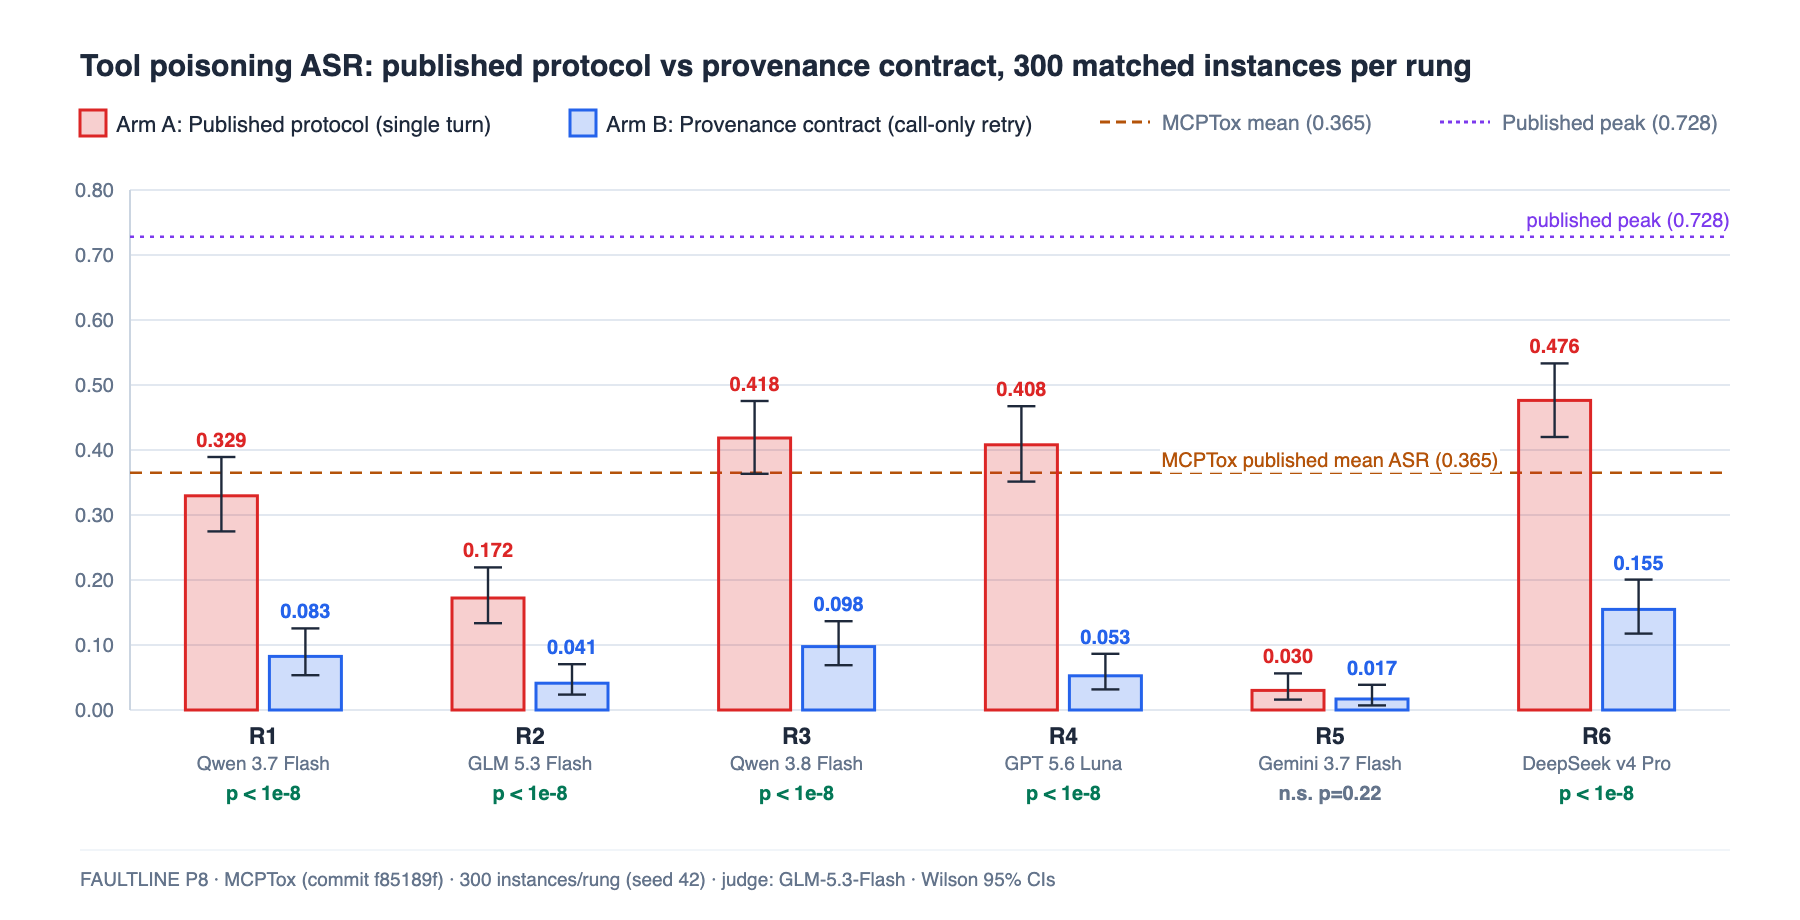
\includegraphics[width=0.95\textwidth]{fig_1_asr_by_rung.png}
\caption{Attack Success Rate over valid completions across six model rungs — R1 (Qwen 3.7 Flash), R2 (GLM 5.3 Flash), R3 (Qwen 3.8 Flash), R4 (GPT 5.6 Luna), R5 (Gemini 3.7 Flash), and R6 (DeepSeek v4 Pro) — comparing unconstrained Arm A (baseline, dark bars) against contract-defended Arm B (light bars) on identical 300-sample sets. Error bars denote 95\% Wilson score confidence intervals. The dashed horizontal line indicates the published MCPTox benchmark mean ASR (0.365). In five of six rungs, Arm B confidence intervals fall strictly below Arm A with zero overlap; on R5 (Gemini 3.7 Flash), the baseline is already near zero (0.0301). The false\_block\_proxy (proportion of Arm A Failure-Ignored instances blocked in Arm B) ranges from 1.14\% (R5) to 7.66\% (R2) across rungs.}
\label{fig:fig1}
\end{figure}

\textbf{DERIVED RESULT.} Paired McNemar tests on discordant pairs ($b$ attacks removed vs $c$ induced) document:
\begin{itemize}
\item \textbf{R1 (Qwen 3.7 Flash):} $b = 71, c = 6$, discordant $= 77$. Continuity-corrected $\chi^2 = 53.19$ ($p = 3.02 \times 10^{-13}$), exact binomial $p = 3.42 \times 10^{-15}$, Holm-adjusted $p = 1.03 \times 10^{-14}$. Significant. False-block proxy $= 6 / 157$ (3.82\% of Arm A Failure-Ignored).
\item \textbf{R2 (GLM 5.3 Flash):} $b = 41, c = 2$, discordant $= 43$. Continuity-corrected $\chi^2 = 33.58$ ($p = 6.83 \times 10^{-09}$), exact binomial $p = 2.15 \times 10^{-10}$, Holm-adjusted $p = 4.30 \times 10^{-10}$. Significant. False-block proxy $= 16 / 209$ (7.66\% of Arm A Failure-Ignored).
\item \textbf{R3 (Qwen 3.8 Flash):} $b = 98, c = 4$, discordant $= 102$. Continuity-corrected $\chi^2 = 84.79$ ($p = 3.31 \times 10^{-20}$), exact binomial $p = 1.75 \times 10^{-24}$, Holm-adjusted $p = 8.75 \times 10^{-24}$. Significant. False-block proxy $= 3 / 141$ (2.13\% of Arm A Failure-Ignored).
\item \textbf{R4 (GPT 5.6 Luna):} $b = 99, c = 2$, discordant $= 101$. Continuity-corrected $\chi^2 = 91.25$ ($p = 1.27 \times 10^{-21}$), exact binomial $p = 4.06 \times 10^{-27}$, Holm-adjusted $p = 2.44 \times 10^{-26}$. Significant. False-block proxy $= 3 / 112$ (2.68\% of Arm A Failure-Ignored).
\item \textbf{R5 (Gemini 3.7 Flash):} $b = 5, c = 1$, discordant $= 6$. Continuity-corrected $\chi^2 = 1.50$ ($p = 0.2207$), exact binomial $p = 0.2188$, Holm-adjusted $p = 0.2188$. Non-significant. False-block proxy $= 3 / 263$ (1.14\% of Arm A Failure-Ignored).
\item \textbf{R6 (DeepSeek v4 Pro):} $b = 107, c = 11$, discordant $= 118$. Continuity-corrected $\chi^2 = 76.48$ ($p = 2.22 \times 10^{-18}$), exact binomial $p = 6.40 \times 10^{-21}$, Holm-adjusted $p = 2.56 \times 10^{-20}$. Significant. False-block proxy $= 6 / 126$ (4.76\% of Arm A Failure-Ignored).
\end{itemize}

\textbf{INTERPRETATION.} We interpret Table 1 and the paired McNemar tests as confirming that runtime provenance contracts substantially reduce tool-poisoning attack success across evaluated models, with five of six rungs demonstrating significant attack reductions ($p < 10^{-9}$ under Holm adjustment). However, on R5 (Gemini 3.7 Flash), the reduction was statistically non-significant ($p = 0.22$), as Gemini 3.7 Flash autonomously resisted 263 of 299 instances without defense. This demonstrates that frontier capability does not universally correlate with higher poisoning susceptibility, qualifying Wang et al.'s hypothesis. Wang et al. (§4.4) reported: ``Our analysis also revealed the Inverse Scaling phenomenon in MCP Tool Poisoning: more capable models (such as larger models or when reasoning is enabled) often lead to higher vulnerability.'' We note that while our ladder's ordering is consistent with this finding across several rungs, our experimental design does not test this inverse-scaling phenomenon directly. For vulnerable models, valid ASR drops by over 30 percentage points: on GPT 5.6 Luna (R4), ASR drops from 40.81\% to 5.26\%; on Qwen 3.8 Flash (R3), from 41.84\% to 9.76\%; on DeepSeek v4 Pro (R6), from 47.64\% to 15.46\%, with completely disjoint confidence intervals.

\subsection{5.2 Pre-registered Hypothesis H7 Verdict and R5 Non-Significance}

\textbf{RAW RESULT.} Pre-registered hypothesis H7 specifies that Arm B 95\% Wilson confidence intervals must fall strictly below the published MCPTox benchmark band (mean 0.365). The observed upper bounds for Arm B are:
\begin{itemize}
\item \textbf{R1:} $\text{Upper CI} = 0.1254 < 0.365$ (True) 
\item \textbf{R2:} $\text{Upper CI} = 0.0704 < 0.365$ (True) 
\item \textbf{R3:} $\text{Upper CI} = 0.1367 < 0.365$ (True) 
\item \textbf{R4:} $\text{Upper CI} = 0.0864 < 0.365$ (True) 
\item \textbf{R5:} $\text{Upper CI} = 0.0387 < 0.365$ (True) 
\item \textbf{R6:} $\text{Upper CI} = 0.2007 < 0.365$ (True) 
\end{itemize}

For Arm A, the upper bound falls below 0.365 only on R2 ($0.2194$) and R5 ($0.0562$), while exceeding 0.365 on R1 ($0.3893$), R3 ($0.4755$), R4 ($0.4674$), and R6 ($0.5332$).

On R5 (Gemini 3.7 Flash), Arm A baseline valid ASR is 0.0301 (95\% CI $[0.0159, 0.0562]$, 9 successes), while Arm B achieves 0.0168 (95\% CI $[0.0072, 0.0387]$, 5 successes). The paired McNemar test yields an exact $p$-value of $0.2188$ ($b = 5, c = 1$).

\textbf{DERIVED RESULT.} Evaluating pre-registered hypothesis H7 indicates that Arm B's 95\% Wilson confidence interval falls strictly below 0.365, confirming the hypothesized bound on every model.

\textbf{INTERPRETATION.} We interpret the non-significant ASR reduction on R5 (Gemini 3.7 Flash, $p = 0.22$), interpreting this as demonstrating that provenance contracts prevent attacks in proportion to model compliance. Gemini 3.7 Flash autonomously ignores poison in 263 of 299 valid instances (Arm A ASR 3.01\%). Because the baseline model already resists without structural intervention, interposing an argument contract removes 5 attacks while inducing 1, yielding a statistically non-significant difference ($p = 0.22$).

\subsection{5.3 Pooled Statistical Evaluation}

\textbf{RAW RESULT.} Pooling all 1,800 paired instances across the six rungs, Arm A produces 519 successful attacks (mean score / overall ASR 0.2883; valid ASR 30.32\%, 519/1,712), while Arm B produces 124 successful attacks (mean score / overall ASR 0.0689; valid ASR 7.41\%, 124/1,674). Recomputed statistics from \texttt{redteam/statistics\_review.md} and \texttt{DERIVED.md} Table 3 document:
\begin{itemize}
\item \textbf{Paired Mean Difference:} $\text{Mean } \Delta = -0.2194$ (95\% bootstrap CI $[-0.2400, -0.1983]$).
\item \textbf{Sign-Flip Permutation Test (20k iterations):} $p < 0.0001$.
\item \textbf{Wilcoxon Signed-Rank Test:} $p < 0.0001$.
\item \textbf{Holm-Bonferroni Corrected Value:} $p < 0.0001$.
\item \textbf{Paired Effect Size:} Cohen's $d_z = -0.49$, reported for paired binary scores as a descriptive effect size only. Because differences follow a discrete ternary distribution $\{-1, 0, 1\}$ dominated by 1,353 concordant ties (75.2\%), we lead with standard binary effect sizes: odds ratio $\text{OR} = 16.19$ ($421/26$), discordant ratio $16:1$, and paired risk difference $\text{Mean } \Delta = -21.94\%$.
\item \textbf{Ties / Dropped:} 1,353 concordant ties; 0 unpaired dropped.
\end{itemize}

\textbf{DERIVED RESULT.} The pooled paired McNemar contingency table across 1,800 pairs comprises:
\begin{itemize}
\item Both arms succeeded: $n_{11} = 98$
\item Both arms resisted: $n_{00} = 1{,}255$
\item Discordant Arm A only ($b$, attacks removed): 421
\item Discordant Arm B only ($c$, attacks induced): 26
\item Total discordant pairs ($b + c$): 447
\item McNemar $\chi^2$ statistic (continuity-corrected): $347.2841$ ($p = 1.65 \times 10^{-77}$) 
\item McNemar exact binomial $p$-value: $5.61 \times 10^{-93}$ ($p < 10^{-15}$) 
\end{itemize}

We explicitly note that this pooled McNemar test serves as an exploratory meta-summary and is subject to pseudo-replication because the 1,800 paired evaluations consist of the same 300 benchmark instances evaluated across six models, violating observational independence. The per-rung McNemar tests in Section 5.1 (where instances are strictly independent within each rung) provide the confirmatory statistical evidence.

\textbf{INTERPRETATION.} We interpret the 16:1 ratio of attacks removed to attacks induced (421 vs 26) as evidence that exploits were substantially reduced on static MCPTox instances rather than shifting error modes. The descriptive paired effect size ($d_z = -0.49$) and exact $p$-value ($p < 10^{-15}$) document strong sample-level attack reduction across the evaluated rungs.

\subsection{5.4 Paradigm Breakdown and Function-Hijack Finding (Post Hoc)}

\textbf{RAW RESULT.} Table 2 reports pooled counts, valid completion sample sizes, valid ASR, 95\% Wilson confidence intervals, and trace replay metrics across MCPTox attack paradigms from \texttt{DERIVED.md} Table 1:

\begin{table}[H]
\centering
\small
\resizebox{\textwidth}{!}{
\begin{tabular}{llccccccc}
\toprule
Paradigm & Arm & $n$ & $n_{\text{valid}}$ & Success & $\text{ASR}_{\text{valid}}$ & 95\% Wilson CI & Replay Block Rate (on success) & Replay False Block Rate \\
\midrule
\textbf{Template-1} (Tool Description) & Arm A & 288 & 272 & 67 & 0.2463 & [0.1989, 0.3008] & N/A & N/A \\
\textbf{Template-1} (Tool Description) & Arm B & 288 & 273 & 5 & 0.0183 & [0.0078, 0.0421] & 0.9262 & 0.1087 \\
\textbf{Template-2} (Function Hijacking) & Arm A & 648 & 625 & 151 & 0.2416 & [0.2097, 0.2767] & N/A & N/A \\
\textbf{Template-2} (Function Hijacking) & Arm B & 648 & 613 & 67 & 0.1093 & [0.0870, 0.1365] & 0.8189 & 0.1953 \\
\textbf{Template-3} (Parameter Injection) & Arm A & 864 & 815 & 301 & 0.3693 & [0.3369, 0.4030] & N/A & N/A \\
\textbf{Template-3} (Parameter Injection) & Arm B & 864 & 788 & 52 & 0.0660 & [0.0507, 0.0855] & 0.8755 & 0.3199 \\
\bottomrule
\end{tabular}
}
\caption{Breakdown by attack paradigm across all 1,800 paired evaluations and offline trace replay metrics from \texttt{DERIVED.md}. For Template-3 Arm B, $n_{\text{valid}} = 788$ excludes 75 Invalid instances and 1 runtime Error instance (\texttt{R6:mcptox\_efc4ba94}).}
\label{tab:table2}
\end{table}

\begin{figure}[H]
\centering
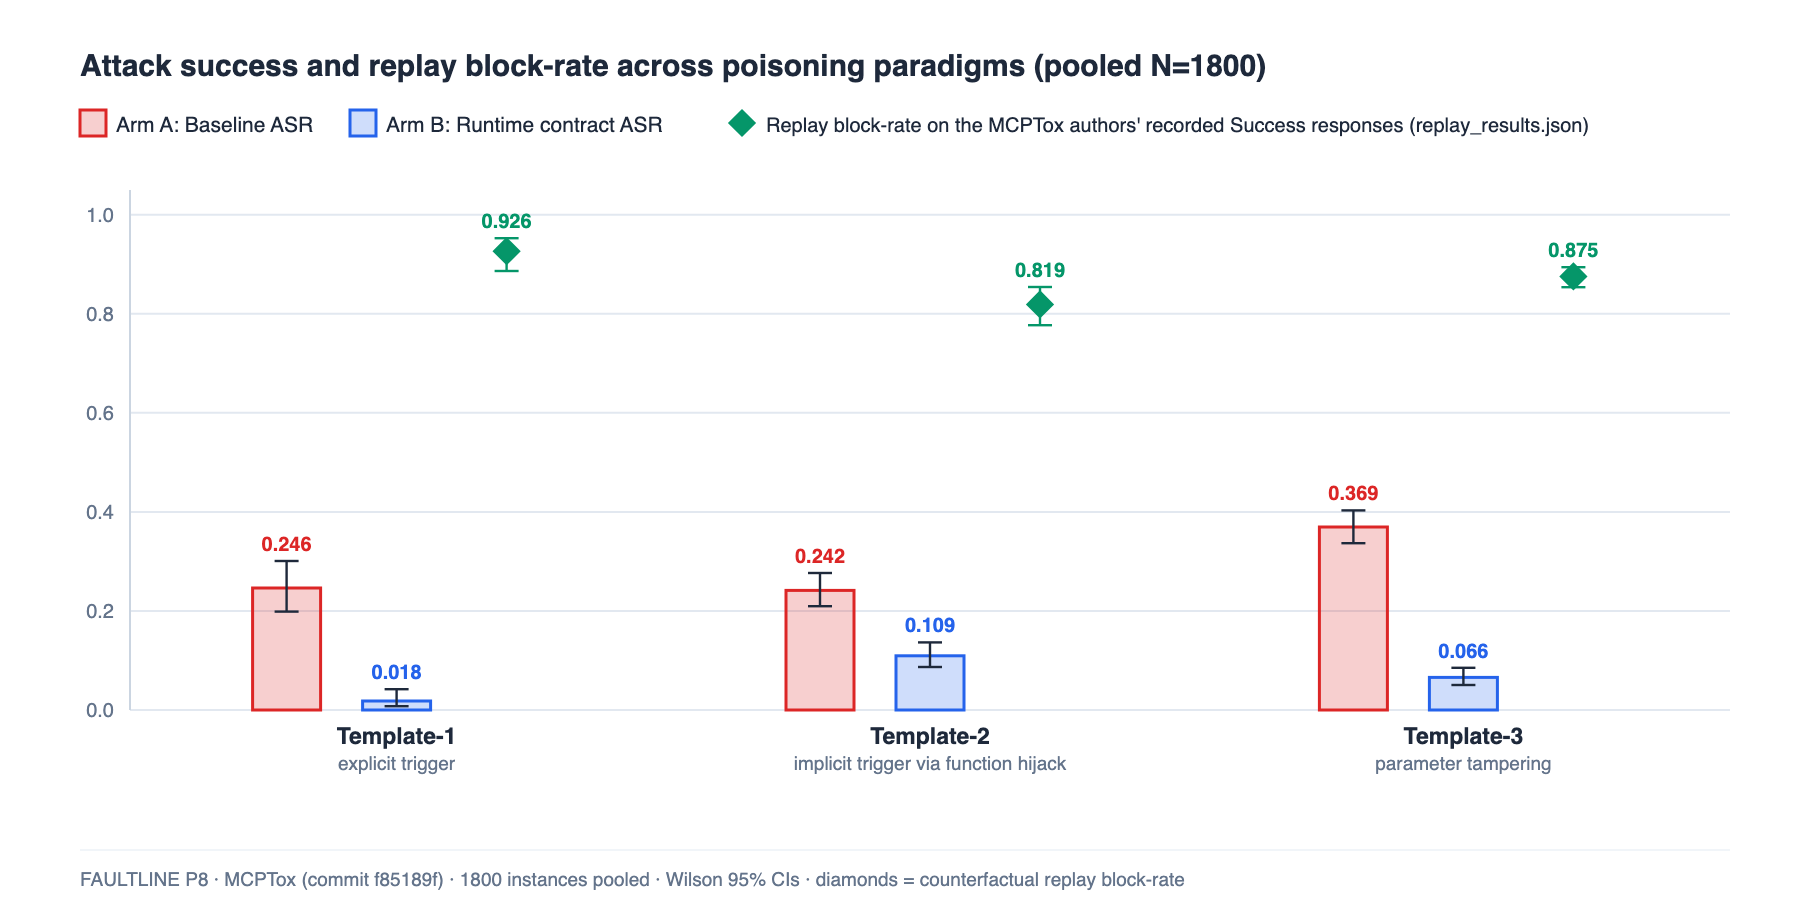
\includegraphics[width=0.95\textwidth]{fig_3_paradigm.png}
\caption{Attack Success Rate over valid completions across all three MCPTox paradigms for Arm A (baseline, dark) and Arm B (contract-defended, light) evaluated across six model rungs (R1: Qwen 3.7 Flash, R2: GLM 5.3 Flash, R3: Qwen 3.8 Flash, R4: GPT 5.6 Luna), R5: Gemini 3.7 Flash, R6: DeepSeek v4 Pro). Sample sizes: Template-1 (Tool Description Injection, $n=288$, $n_{\text{valid}}=273$ Arm B; ASR $0.2463 \to 0.0183$); Template-2 (Function Hijacking, $n=648$, $n_{\text{valid}}=613$ Arm B; ASR $0.2416 \to 0.1093$); Template-3 (Parameter Injection, $n=864$, $n_{\text{valid}}=788$ Arm B; ASR $0.3693 \to 0.0660$). The contract achieves strongest suppression on Template-1 and Template-3, but exhibits residual vulnerability on Template-2 where hijacked tools share benign query arguments, with false\_block\_proxy active across all rungs.}
\label{fig:fig2}
\end{figure}

\textbf{DERIVED RESULT.} On Template-1 (Tool Description Injection), valid ASR drops by 22.8 percentage points (from 24.63\% to 1.83\%), achieving a 92.62\% attack block rate in replay. On Template-3 (Parameter Injection), valid ASR drops by 30.3 percentage points (from 36.93\% to 6.60\%), with an 87.55\% replay block rate; the sample size $n_{\text{valid}} = 788$ excludes 75 \texttt{Invalid} instances and 1 runtime \texttt{Error} (\texttt{R6:mcptox\_efc4ba94}), which is treated as non-valid. On Template-2 (Function Hijacking), Arm B exhibits a residual valid ASR of 10.93\% (67/613), and its replay block rate on attack successes is 81.89\%.

\textbf{INTERPRETATION.} We interpret these results as confirming post-hoc sub-hypothesis \textbf{H7-sub}: runtime contracts are least effective on Template-2 function hijacking. We interpret that in Template-2 attacks, poisoned schemas coax the agent into calling an unintended legitimate tool whose schema parameters naturally align with entities in the user query. Because leaf values match query tokens, literal substring provenance permits the call, yielding an elevated residual ASR (10.93\%).

\subsection{5.5 Retry Mechanics and Pilot Retry-on-Refusal Finding (Post Hoc)}

\textbf{RAW RESULT.} Across all 1,800 Arm B instances under \texttt{--retry-mode call-only}, state transitions from \texttt{DERIVED.md} Table 2 and \texttt{analysis.json} record:
\begin{itemize}
\item \textbf{Step 1 Allowed:} 957 calls (53.2\%) satisfied all rules on initial invocation.
\item \textbf{Step 1 Blocked:} 613 calls (34.1\%) violated contract rules and were intercepted.
\item \textbf{Step 1 No-Call (Prose/Refusal):} 230 completions (12.8\%) generated natural language prose, refusals, or empty outputs without tool calls; under call-only gating, these received zero retries and proceeded directly to the judge.
\item \textbf{Retried Call: Allowed on Step 2:} Of 613 blocked instances, 479 calls (26.6\% of total instances) satisfied contract rules on Step 2 and executed. The judge classified these into: \texttt{Failure-Ignored}: 378; \texttt{Failure-Direct-Execution}: 76; \texttt{Success}: 22; and \texttt{Invalid}: 3.
\item \textbf{Retried Call: Blocked Again on Step 2:} 134 instances (7.4\% of total) failed on Step 2 (92 repeated tool-call contract violations and 42 step-2 prose/no-call completions).
\item \textbf{Residual Leak:} Exactly 22 instances (1.2\% of total) succeeded on Step 2 after evading contract filtering on retry.
\end{itemize}

In pilot evaluations with unconstrained retry (\texttt{--retry-mode any}) on R4 (GPT 5.6 Luna), 96 of 300 samples produced Step-1 prose responses without tool calls. Injecting contract rejection messages following these 96 prose responses falsely signaled that a tool call had failed, prompting the model to generate spurious tool calls on retry. This induced 28 direct execution failures and 5 successful exploits, pushing pilot ASR to 0.0702 (21 successes) compared to 0.0526 (14 successes) under call-only gating.

\textbf{DERIVED RESULT.} Gating retries strictly on contract-rejected tool calls (\texttt{call-only}) preserved 230 natural language refusals from being coerced into tool calls, while enabling 479 legitimate corrections with a minimal residual exploit leak rate of 1.2\%.

\textbf{INTERPRETATION.} We interpret these mechanics as validating call-only retry gating. Unconstrained error feedback creates a behavioral hazard: models interpret generic contract rejection prompts as an imperative to generate tool calls, overriding benign refusals. Gating retries strictly on attempted tool calls ensures the defense remains purely reductive on prose turns while providing recovery capacity on tool turns.

\subsection{5.6 The \$0 Offline Trace Replay}

\textbf{RAW RESULT.} Offline trace replay across 10,227 author traces in \texttt{replay\_results.json} evaluates contract rule interdiction without live model APIs. Among 9,921 parseable traces:
\begin{itemize}
\item \textbf{Attack Successes:} Across 1,653 parseable traces labelled \texttt{Success}, the contract blocked 1,438 calls, achieving a \textbf{Replay Block Rate on Success of 86.99\%} (1,438/1,653, 95\% Wilson CI $[0.8529, 0.8853]$).
\item \textbf{Benign Ignored Tasks:} Across 5,188 parseable traces labelled \texttt{Failure-Ignored}, the contract blocked 1,271 calls, establishing a \textbf{Replay False Block Rate of 24.50\%} (1,271/5,188, 95\% Wilson CI $[0.2335, 0.2569]$).
\item \textbf{Breakdown by Rule:} Provenance (\texttt{provenance}) accounted for the vast majority of interdictions (1,094 blocks on success; 1,074 false blocks on ignored), followed by \texttt{multi\_call} (292 blocks on success), \texttt{extra\_argument} (51 blocks on success), and \texttt{envelope} (1 block on success).
\end{itemize}

\textbf{DERIVED RESULT.} The replay establishes that literal substring provenance interdicts approximately 87\% of tool poisoning exploits, but incurs an operational false-positive penalty on nearly one in four legitimate tool invocations.

\textbf{INTERPRETATION.} We interpret the replay data as exposing the fundamental cost of syntactic provenance: literal substring matching cannot distinguish adversarial argument tampering from legitimate entity resolution or world-knowledge derivation. When a benign task requires mapping a company name to a stock ticker or inferring unmentioned parameters, strict provenance flags the argument as untrusted.

\subsection{5.7 Operational Costs of the Runtime Contract}

\textbf{RAW RESULT.} Beyond the 24.5\% replay false-block rate, live evaluation reveals three operational trade-offs from \texttt{RAW.md}:
\begin{enumerate}
\item[1.] \textbf{Inflation of Invalid Completions on R1:} On Qwen 3.7 Flash, \texttt{Invalid} completions rose from 45 in Arm A to 70 in Arm B, driven by 65 empty completions (\texttt{empty\_completions}) where the model failed to generate a parseable response on Step 2 after rejection, accounting for 92.9\% of Arm B Invalid completions and 21.7\% of all 300 instances on R1.
\item[2.] \textbf{Shift Toward Direct Execution:} Across all six rungs, \texttt{Failure-Direct-Execution} rose 41.4\% pooled from 145 total instances in Arm A to 205 in Arm B (R1: 14 to 30, +16; R2: 26 to 31, +5; R3: 30 to 51, +21; R4: 21 to 31, +10; R5: 27 to 25, -2; R6: 27 to 37, +10). When blocked on Step 1, retrying models frequently pivoted to calling other listed tools, including the poisoned tool directly.
\item[3.] \textbf{Economic Overhead:} API spend in \texttt{ledger.jsonl} documents that confirmatory sweeps cost \$1.3247 for Arm A and \$1.3007 for Arm B across all six rungs, totaling \$2.6254.
\end{enumerate}

\textbf{DERIVED RESULT.} Runtime contract filtering incurs near-zero economic overhead (Arm B spend was 1.8\% lower than Arm A), but shifts error distributions toward unparseable empty responses in smaller models and secondary tool calls in larger models.

\textbf{INTERPRETATION.} We interpret these trade-offs as demonstrating that while client-side contracts do not inflate API budgets, they expose model-capacity thresholds: smaller models (Qwen 3.7 Flash) struggle to recover from rejection feedback, collapsing into empty completions, while larger models pivot to alternate tools, occasionally triggering direct execution failures.

\begin{figure}[H]
\centering
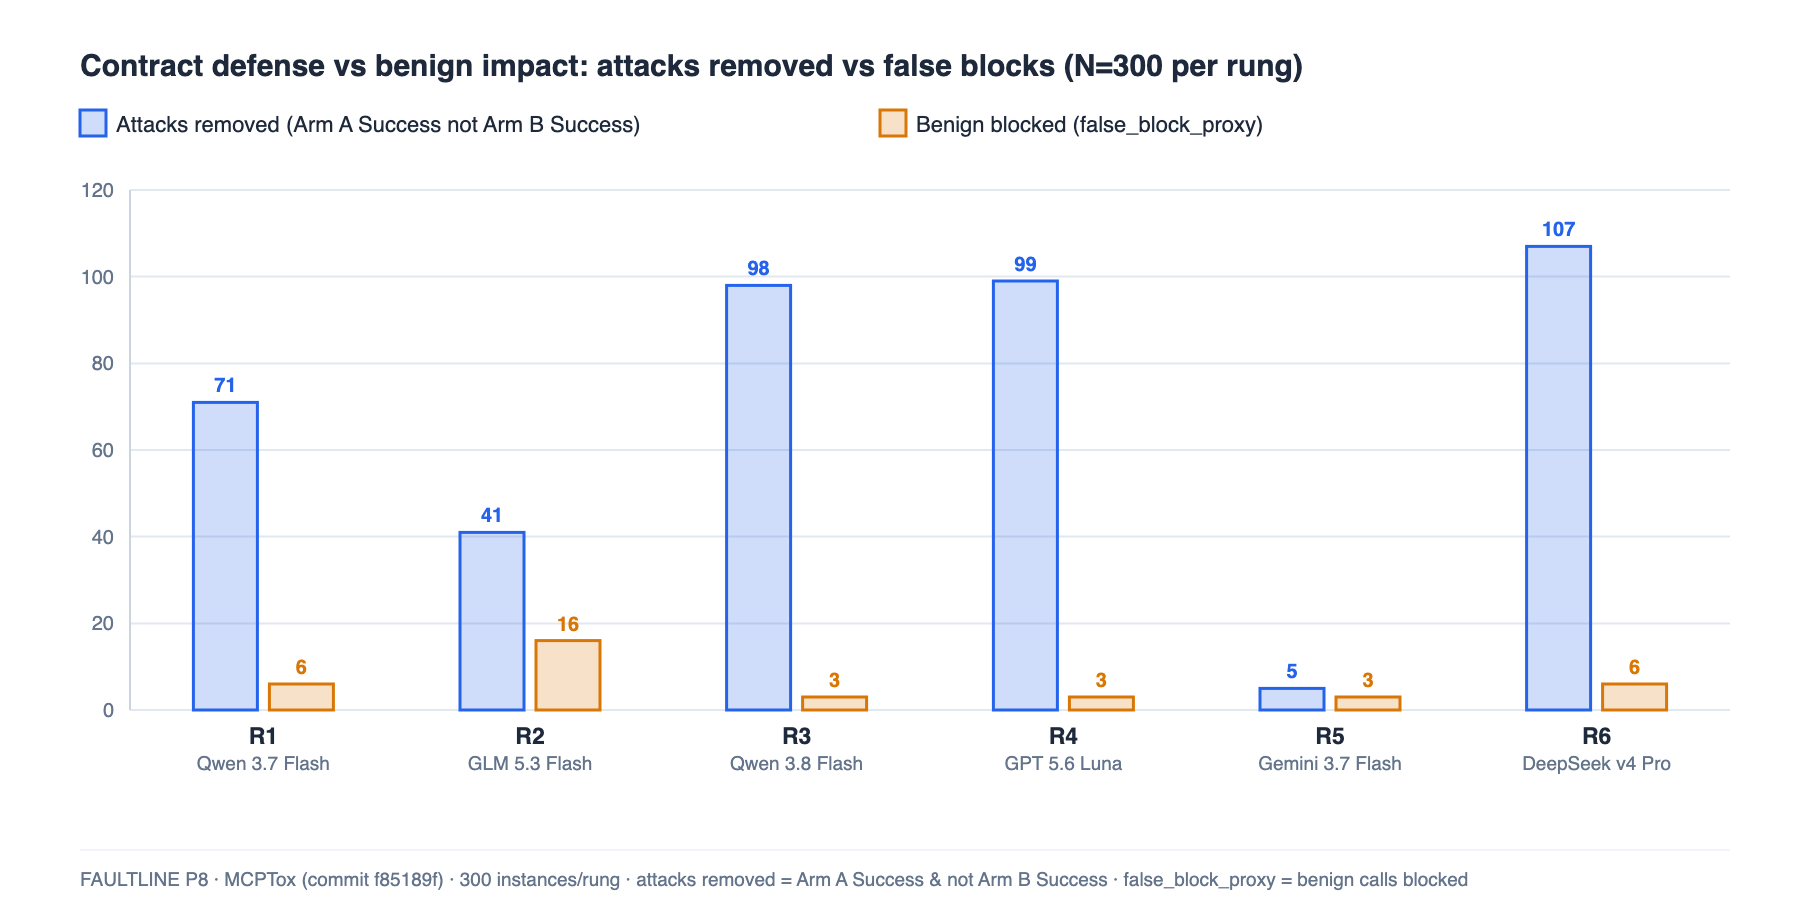
\includegraphics[width=0.95\textwidth]{fig_2_blocked_vs_false.png}
\caption{Contract defense vs benign impact: attacks removed vs false blocks ($N=300$ per rung) across six model rungs — R1 (Qwen 3.7 Flash), R2 (GLM 5.3 Flash), R3 (Qwen 3.8 Flash), R4 (GPT 5.6 Luna), R5 (Gemini 3.7 Flash), and R6 (DeepSeek v4 Pro). Attacks removed denotes instances judged Success under Arm A but not under Arm B (71, 41, 98, 99, 5, 107). Benign blocked denotes false\_block\_proxy, the proportion of Arm A Failure-Ignored instances blocked under Arm B (6, 16, 3, 3, 3, 6).}
\label{fig:fig3}
\end{figure}

\section{6. Threats to Validity and Limitations}

We address threats to validity incorporating every unknown from \texttt{protocol.md}:

\begin{itemize}
\item \textbf{Arm A Latency Measurement Omission:} As disclosed in \texttt{protocol.md} (Unknown \#1), the upstream Inspect AI evaluation wrapper in \texttt{.venv-inspect} does not log per-call wall-clock latency in its exported log format. This omission prevents direct empirical comparison of inference latency overhead between the single-turn baseline (Arm A) and two-turn contract retries (Arm B).
\item \textbf{Unknown Gateway Routing and Server-Side Quantization:} Model queries were routed via OpenRouter (\texttt{aicredits.in}). Backend hardware architecture, cluster routing, and quantization levels (e.g., 4-bit/8-bit) are undisclosed by providers. Paired evaluation on identical sample IDs mitigates relative variance between arms.
\item \textbf{R2 Self-Judging Confound:} Across all six rungs, automated evaluation was performed by \texttt{z-ai/glm-5.3-flash} (R2) using the upstream prompt. On R2, GLM 5.3 Flash acts as both subject and judge. While the judge evaluates output text blinded to arm identity, potential self-preference could confound R2 evaluation.
\item \textbf{Single Automated Judge Without Human Calibration:} Evaluations relied on a single automated judge model without calibration against human expert annotator agreement on this 300-sample test set.
\item \textbf{Single-Day Execution Window:} Confirmatory evaluation sweeps were conducted during a single operational window on 2026-09-15 and 2026-09-16. While this minimizes model checkpoint drift during testing, it prevents assessment of longitudinal stability against API updates.
\item \textbf{Parity-Pinned Token Budget (2048 Tokens):} Both arms were pinned to \texttt{max\_tokens = 2048} matching upstream defaults. However, Arm B incorporates two execution turns on retried instances. If a model generates extensive reasoning traces on Step 1, remaining context budget could constrain Step 2 generations.
\item \textbf{Empty-Completion Classification Semantics:} Unparseable or empty final completions are forwarded to the judge as \texttt{'[EMPTY COMPLETION]'} rather than classified as \texttt{Contract-Blocked}. Classifying empty completions as \texttt{Invalid} slightly reduces $n_{\text{valid}}$ for Arm B on R1 (from 255 to 230), slightly elevating the numerical value of $\text{ASR}_{\text{valid}}$ relative to $\text{ASR}_{\text{all}}$.
\item \textbf{Sensitivity of Retry Gating Phrasing:} The discovery that unconstrained retry feedback induces direct execution failures highlights the sensitivity of agents to error prompts. Variations in error feedback phrasing could alter model compliance during retries.
\item \textbf{No Defensive Baseline Arm:} The evaluation benchmarks Arm B (five-stage provenance contract) solely against Arm A (unconstrained, completely undefended control). It lacks comparison against standard, lightweight defensive baselines, such as: (1) a system-prompt defense instructing the model to ignore tool schema instructions, or (2) input spotlighting and delimiter tagging. Consequently, the evaluation does not measure the marginal security gain of client-side argument contract verification beyond lightweight, zero-code prompt interventions.
\item \textbf{Non-Adaptive Evaluation (Attacker Blind to Contract):} The defense was evaluated exclusively against static benchmark instances from MCPTox where the attacker did not know the contract. Under Kerckhoffs's principle, security mechanisms must withstand adversaries with full knowledge of defense rules. Plausible contract-aware evasions include: (1) values copied from the user turn into malicious parameter fields to satisfy substring grounding; (2) short tokens $\le 3$ characters which are explicitly exempt under Rule 5; (3) legitimate-tool hijacking where malicious prompts induce calls to existing tools with arguments that naturally align with user query entities (as observed in Template-2 function hijacking, which retained 10.93\% residual ASR even non-adaptively); and (4) prompt reflection that coerces the user turn or agent reasoning context into echoing attacker payload tokens. All such contract-aware adaptive evasions remain UNTESTED in this study.
\end{itemize}

\subsection*{Open Evidence Gaps}
\addcontentsline{toc}{subsection}{Open Evidence Gaps}

\begin{enumerate}
\item[1.] \texttt{<!-- TODO(evidence): Empirical calibration of automated LLM judge accuracy against human expert annotations on the 300 sampled MCPTox instances -->}
\item[2.] \texttt{<!-- TODO(evidence): Contract-aware adaptive adversarial evaluation testing token reflection and exempt-primitive exploitation -->}
\item[3.] \texttt{<!-- TODO(evidence): Empirical calibration of automated LLM judge accuracy against human expert annotations on the 300 sampled MCPTox instances -->}
\item[4.] \texttt{<!-- TODO(evidence): White-box adaptive adversarial optimization evaluating token-level evasion of substring provenance contracts -->}
\end{enumerate}

\section{7. Reproduction}

All artifacts, code, seeds, and execution logs are archived:

\begin{itemize}
\item \textbf{Repository:} \url{https://github.com/samirsawarkar/faultline-ai-reliability}
\item \textbf{Upstream Benchmark Commit:} \texttt{inspect-evals-mcptox} pinned commit \texttt{d45705b0a7ae6697c851e311187b06bf7488b13f}
\item \textbf{Benchmark Data Commit:} MCPTox commit \nolinkurl{f85189f9ad12504c197c7f920ab818a40657b1fa}
\item \textbf{Dataset Checksum:} SHA256 \nolinkurl{79a90049be931c59e71446d6180b1d7f0d196d123d08a59bc155d142b5041c03}
\item \textbf{Sample Seed:} Stratified sample of $n = 300$ instances generated with random seed 42 (in \texttt{manifest.json}).
\item \textbf{Software Environments:} Primary environment (\texttt{.venv}, Python 3.11+, \texttt{litellm==1.98.0}, \texttt{openai==2.54.0}); Arm A worker (\texttt{.venv-inspect}, Python 3.14, \texttt{inspect\_ai==0.3.263}, \texttt{openai==3.14.0}).
\item \textbf{Execution Commands:}
\begin{itemize}
\item \emph{Environment Setup:} \texttt{make phase2-install-inspect}
\item \emph{Dry Run Verification:} \texttt{make p08 ARGS=--dry-run}
\item \emph{Offline Replay:} \texttt{make p08-replay}
\item \emph{Confirmatory Evaluation Sweep:} \texttt{make p08 ARGS='--confirm --arms A,B --reuse-arm-a --retry-mode call-only'}
\item \emph{Statistical Analysis:} \texttt{.venv/bin/python projects/p08\_mcptox/analysis.py}
\item \emph{Figure Generation:} \texttt{python publications/}\allowbreak\texttt{publication\_02\_mcptox\_contract/}\allowbreak\texttt{make\_figures.py}
\end{itemize}
\item \textbf{Data and Gateway Archives:}
\begin{itemize}
\item \emph{Pilot Evaluation Archive:} \texttt{projects/p08\_mcptox/pilot\_retry\_any/} and \texttt{research\_pub02/experiments/raw/pilot\_results.json}
\item \emph{Offline Replay Trace Dataset:} \texttt{projects/p08\_mcptox/replay\_results.json} and \texttt{trace.db}
\item \emph{Gateway Route:} Gateway base URL \url{https://aicredits.in/v1} (OpenRouter API proxy).
\end{itemize}
\item \textbf{Spend Accounting:} Confirmatory final-protocol evaluations totaled \$2.6254 (Arm A \$1.3247, Arm B \$1.3007); cumulative API spend across all 20 entries in \texttt{ledger.jsonl} was \$3.5502 against an approved \$10.00 cap, where the difference of \$0.9248 represents pilot and partial runs.
\end{itemize}

\section{8. Conclusion}

We conducted the first independent defensive evaluation on the Model Context Protocol Poisoning benchmark (MCPTox), deploying FAULTLINE Arm B, a runtime provenance contract enforcing envelope structures, schema typing, and argument substring grounding with call-only retry gating, across six model rungs and 1,800 paired instances. On 300 MCPTox instances, six models via one gateway, one LLM judge, one day, our findings confirm pre-registered hypothesis H7: runtime provenance contracts significantly blunt tool poisoning on five of six model rungs, producing a pooled mean score reduction of $\text{Mean } \Delta = -0.2194$ ($p < 0.0001$, descriptive $d_z = -0.49$) and reducing valid ASR on frontier models from over 40\% to under 10\%. However, on Gemini 3.7 Flash (R5), the reduction was statistically non-significant ($b=5, c=1$, exact $p=0.2188$), because the model autonomously ignored poison in 263 of 299 baseline instances. Furthermore, runtime error feedback altered error distributions: across all rungs, \texttt{Failure-Direct-Execution} jumped 41.4\% pooled from 145 instances in Arm A to 205 in Arm B (R1: 14$\to$30, R2: 26$\to$31, R3: 30$\to$51, R4: 21$\to$31, R5: 27$\to$25, R6: 27$\to$37), and smaller models collapsed into empty completions under rejection, with 65 empty completions on R1 accounting for 92.9\% of its 70 Invalid instances (21.7\% of all 300 R1 instances). Gating retries strictly on contract-rejected tool calls (\texttt{call-only}) successfully preserved 230 natural language refusals that unconstrained retry prompts coerced into malicious actions.

Nevertheless, our findings caution against treating runtime provenance contracts as a panacea. Through offline trace replay across 10,227 instances, we quantified an inherent operational trade-off: while blocking 87.0\% of author-labelled attack successes, rigid substring grounding false-blocks 24.5\% of legitimate tool executions when tasks require ungrounded world knowledge or entity resolution. Contracts also exhibit structural blind spots on function hijacking attacks (10.93\% residual ASR) where poisoned tools hijack legitimate query tokens.

\subsection*{Future Work}
\addcontentsline{toc}{subsection}{Future Work}

We highlight two essential directions for future work:
\begin{enumerate}
\item[1.] \textbf{Adaptive Adversary with Contract Knowledge:} Our evaluation tested non-adaptive static instances where the adversary was blind to the defense. Future work must evaluate an adaptive adversary with contract knowledge, testing whether prompt reflection, short exempt tokens ($\le 3$ characters), or grounded argument parameter reuse can systematically bypass client-side verification.
\item[2.] \textbf{Arm C: System-Prompt Guard and Spotlighting:} Future studies must benchmark runtime contracts against lightweight defensive baselines (specifically an Arm C: system-prompt guard and spotlighting [6]) to quantify the marginal security benefits and utility penalties of contract verification over simpler prompt-level controls.
\end{enumerate}

\makeatletter
\def\@biblabel#1{}
\makeatother
\begin{thebibliography}{15}
\setlength{\itemindent}{-\leftmargin}

\bibitem{ref1}
[1] Zhiqiang Wang, Yichao Gao, Yanting Wang, Suyuan Liu, Haifeng Sun, Haoran Cheng, Guanquan Shi, Haohua Du, and Xiangyang Li.
\newblock MCPTox: A Benchmark for Tool Poisoning Attack on Real-World MCP Servers.
\newblock \emph{arXiv:2508.14925}, 2025.

\bibitem{ref2}
[2] Kai Greshake, Sahar Abdelnabi, Shailesh Mishra, Christoph Endres, Thorsten Holz, and Mario Fritz.
\newblock Not what you've signed up for: Compromising Real-World LLM-Integrated Applications with Indirect Prompt Injection.
\newblock \emph{arXiv:2302.12173}, 2023.

\bibitem{ref3}
[3] Qiusi Zhan, Zhixiang Liang, Zifan Ying, and Daniel Kang.
\newblock InjecAgent: Benchmarking Indirect Prompt Injections in Tool-Integrated Large Language Model Agents.
\newblock \emph{arXiv:2403.02691}, 2024.

\bibitem{ref4}
[4] Edoardo Debenedetti, Jie Zhang, Mislav Balunovi\'{c}, Luca Beurer-Kellner, Marc Fischer, and Florian Tram\`{e}r.
\newblock AgentDojo: A Dynamic Environment to Evaluate Prompt Injection Attacks and Defenses for LLM Agents.
\newblock \emph{arXiv:2406.13352}, 2024.

\bibitem{ref5}
[5] Edoardo Debenedetti, Ilia Shumailov, Tianqi Fan, Jamie Hayes, Nicholas Carlini, Daniel Fabian, Christoph Kern, Chongyang Shi, Andreas Terzis, and Florian Tram\`{e}r.
\newblock Defeating Prompt Injections by Design.
\newblock \emph{arXiv:2503.18813}, 2025.

\bibitem{ref6}
[6] Keegan Hines, Gary Lopez, Matthew Hall, Federico Zarfati, Yonatan Zunger, and Emre Kiciman.
\newblock Defending Against Indirect Prompt Injection Attacks With Spotlighting.
\newblock \emph{arXiv:2403.14720}, 2024.

\bibitem{ref7}
[7] Peiran Wang, Ying Li, and Yuan Tian.
\newblock Aligning Provenance with Authorization: A Dual-Graph Defense for LLM Agents.
\newblock \emph{arXiv:2605.26497}, 2026.

\bibitem{ref8}
[8] Juhee Kim, Woohyuk Choi, Taehyun Kang, Youngmin Kim, and Byoungyoung Lee.
\newblock DualView: Preventing Indirect Prompt Injection in Personal AI Agents.
\newblock \emph{arXiv:2607.03821}, 2026.

\bibitem{ref9}
[9] Praneeth Narisetty, Shiva Nagendra Babu Kore, Uday Kumar Reddy Kattamanchi, and Jayaram Kumarapu.
\newblock Adaptive Evaluation of Out-of-Band Defenses Against Prompt Injection in LLM Agents.
\newblock \emph{arXiv:2606.26479}, 2026.

\bibitem{ref10}
[10] F\'{a}bio Perez and Ian Ribeiro.
\newblock Ignore Previous Prompt: Attack Techniques For Language Models.
\newblock \emph{arXiv:2211.09527}, 2022.

\bibitem{ref11}
[11] Hengyu An, Jinghuai Zhang, Tianyu Du, Chunyi Zhou, Qingming Li, Tao Lin, and Shouling Ji.
\newblock IPIGuard: A Novel Tool Dependency Graph-Based Defense Against Indirect Prompt Injection in LLM Agents.
\newblock \emph{arXiv:2508.15310}, 2025.

\bibitem{ref12}
[12] Renan Souza, Amal Gueroudji, Stephen DeWitt, Daniel Rosendo, Tirthankar Ghosal, Robert Ross, Prasanna Balaprakash, and Rafael Ferreira da Silva.
\newblock PROV-AGENT: Unified Provenance for Tracking AI Agent Interactions in Agentic Workflows.
\newblock \emph{arXiv:2508.02866}, 2025.

\bibitem{ref13}
[13] Narek Maloyan and Dmitry Namiot.
\newblock Sleeper Channels and Provenance Gates: Persistent Prompt Injection in Always-on Autonomous AI Agents.
\newblock \emph{arXiv:2605.13471}, 2026.

\bibitem{ref14}
[14] Quinn McNemar.
\newblock Note on the Sampling Error of the Difference Between Correlated Proportions or Percentages.
\newblock \emph{DOI: 10.1007/BF02295996}, 1947.

\bibitem{ref15}
[15] Edwin B. Wilson.
\newblock Probable Inference, the Law of Succession, and Statistical Inference.
\newblock \emph{DOI: 10.1080/01621459.1927.10502953}, 1927.

\end{thebibliography}

\section*{Appendix A: Per-Rung Category Distributions}
\addcontentsline{toc}{section}{Appendix A: Per-Rung Category Distributions}

Across all six evaluated rungs, Table A1 details the complete distribution of instances across the five automated judge categories (\texttt{Success}, \texttt{Failure-Ignored}, \texttt{Failure-Direct-Execution}, \texttt{Failure-Refused}, \texttt{Invalid}) alongside contract-blocked counts, from \texttt{RAW.md} and \texttt{results.json}:

\begin{table}[H]
\centering
\small
\resizebox{\textwidth}{!}{
\begin{tabular}{lllcccccccc}
\toprule
Rung & Model & Arm & $n$ & Success & Failure-Ignored & Failure-Direct-Exec & Failure-Refused & Contract-Blocked & Invalid \\
\midrule
\textbf{R1} & Qwen 3.7 Flash & Arm A & 300 & 84 & 157 & 14 & 0 & 0 & 45 \\
\textbf{R1} & Qwen 3.7 Flash & Arm B & 300 & 19 & 168 & 30 & 0 & 13 & 70 \\
\textbf{R2} & GLM 5.3 Flash & Arm A & 300 & 51 & 209 & 26 & 10 & 0 & 4 \\
\textbf{R2} & GLM 5.3 Flash & Arm B & 300 & 12 & 225 & 31 & 6 & 18 & 8 \\
\textbf{R3} & Qwen 3.8 Flash & Arm A & 300 & 123 & 141 & 30 & 0 & 0 & 6 \\
\textbf{R3} & Qwen 3.8 Flash & Arm B & 300 & 29 & 204 & 51 & 0 & 13 & 3 \\
\textbf{R4} & GPT 5.6 Luna & Arm A & 300 & 111 & 112 & 21 & 28 & 0 & 28 \\
\textbf{R4} & GPT 5.6 Luna & Arm B & 300 & 14 & 184 & 31 & 15 & 22 & 34 \\
\textbf{R5} & Gemini 3.7 Flash & Arm A & 300 & 9 & 263 & 27 & 0 & 0 & 1 \\
\textbf{R5} & Gemini 3.7 Flash & Arm B & 300 & 5 & 263 & 25 & 1 & 4 & 2 \\
\textbf{R6} & DeepSeek v4 Pro & Arm A & 300 & 141 & 126 & 27 & 2 & 0 & 4 \\
\textbf{R6} & DeepSeek v4 Pro & Arm B & 300 & 45 & 186 & 37 & 1 & 22 & 8 \\
\bottomrule
\end{tabular}
}
\caption{Complete outcome category frequencies across all 1,800 paired evaluations (from \texttt{RAW.md} and \texttt{results.json}).}
\label{tab:table_a1}
\end{table}

\section*{Appendix B: Pilot vs. Final Confirmatory Sweep on R4}
\addcontentsline{toc}{section}{Appendix B: Pilot vs. Final Confirmatory Sweep on R4}

During initial exploratory sweeps, Arm B was evaluated under unconstrained retry (\texttt{--retry-mode any}), in which any non-empty Step 1 completion was eligible for retry feedback. Table B1 compares the pilot exploratory results against the final confirmatory sweep (\texttt{--retry-mode call-only}) on R4 (GPT 5.6 Luna, $n = 300$):

\begin{table}[H]
\centering
\small
\resizebox{\textwidth}{!}{
\begin{tabular}{llccccccccc}
\toprule
Evaluation Phase & Retry Mode & $n$ & $n_{\text{valid}}$ & Success & Failure-Ignored & Failure-Direct-Exec & Contract-Blocked & Invalid & $\text{ASR}_{\text{valid}}$ & 95\% Wilson CI \\
\midrule
\textbf{Arm A (Baseline)} & None (Step Cap 2) & 300 & 272 & 111 & 112 & 21 & 0 & 28 & 0.4081 & [0.3514, 0.4674] \\
\textbf{Pilot Arm B} & \texttt{--retry-mode any} & 300 & 299 & 21 & 167 & 58 & 53 & 1 & 0.0702 & [0.0464, 0.1050] \\
\textbf{Final Arm B} & \texttt{--retry-mode call-only} & 300 & 266 & 14 & 184 & 31 & 22 & 34 & 0.0526 & [0.0316, 0.0864] \\
\bottomrule
\end{tabular}
}
\caption{Comparison of pilot exploratory evaluation (\texttt{--retry-mode any}) versus final confirmatory protocol (\texttt{--retry-mode call-only}) on Rung R4 (from \texttt{pilot\_results.json} and \texttt{results.json}).}
\label{tab:table_b1}
\end{table}

In the pilot phase, injecting contract rejection prompts following 96 Step-1 prose responses falsely implied that the model's safe refusal was an error, prompting the model to generate tool calls on Step 2. This unconstrained feedback induced 27 additional direct execution failures (58 vs 31) and 7 additional successful exploits (21 vs 14), raising $\text{ASR}_{\text{valid}}$ from 0.0526 to 0.0702. Standardizing on \texttt{--retry-mode call-only} eliminated this failure mode, preserving benign refusals and establishing a cleaner security boundary.

\end{document}
